\documentclass[
  aspectratio=169,
]{beamer}

\usepackage[slovak]{babel}
\usepackage{svg}
\usepackage{listings}
\usepackage[utf8]{inputenc}
\usepackage[T1]{fontenc}
\usepackage{csquotes}
\usepackage{expl3,biblatex}
\addbibresource{example.bib}
\usepackage{booktabs}
\usetheme[
  workplace=fi,
  locale=czech,
]{MU}

\usepackage{listings}
\usepackage{color}

\definecolor{mygreen}{rgb}{0,0.6,0}
\definecolor{mygray}{rgb}{0.5,0.5,0.5}
\definecolor{mymauve}{rgb}{0.58,0,0.82}

\lstset{
  basicstyle=\footnotesize,
  breakatwhitespace=false,
  breaklines=true,
  captionpos=b,
  commentstyle=\color{mygreen},
  deletekeywords={...},
  escapeinside={\%*}{*)},
  extendedchars=true,
  firstnumber=1000,
  frame=none,
  keepspaces=true,
  keywordstyle=\color{blue},
  language=Python,
  morekeywords={*,...},
  numbers=none,
  numbersep=5pt,
  numberstyle=\tiny\color{mygray},
  rulecolor=\color{black},
  showspaces=false,
  showstringspaces=false,
  showtabs=false,
  stepnumber=2,
  stringstyle=\color{mymauve},
  tabsize=4,
  title=\lstname,
}

\title[Structure Quality Control]{Replikácia funkcionality PDB validačného servera v prostredí MetaCentra}
\subtitle[Alternatívny názov prezentácie]{}
\author[M.\, Jediný]{Martin Jediný \\
  Advisor: Mgr. Vladimír Horský, Ph.D.}
\institute[FI MU]{Fakulta informatiky Masarykovej univerzity}
\date{26. júna 2024}
\begin{document}

\begin{frame}[plain]
	\maketitle
\end{frame}

\begin{frame}{Motivácia}{Biomakromolekuly}
	\begin{itemize}
		\item Kľúčovú úloha v rôznych biologických procesoch
		\item Veľmi veľké molekuly --- tisíce a viac opakujúcich sa jednotiek
		      \begin{itemize}
			      \item Bielkoviny
			      \item Nukleové kyseliny
			      \item Polysacharidy
		      \end{itemize}
		\item Funkcia určená štruktúrou
		\item Určenie štruktúry je nevyhnutné pre pochopenie biologických procesov
	\end{itemize}
\end{frame}

\begin{frame}{Motivácia}{Štrukturálne dáta}
	\begin{itemize}
		\item Experimentálne alebo prediktívne metódy (\emph {AlphaFold DB})
		      \begin{itemize}
			      \item Potenciál na vznik chýb
		      \end{itemize}
		\item Uložené ako polohy atómov v trojrozmernom priestore
		\item Nutná validácia výsledných dát
	\end{itemize}
\end{frame}

\begin{frame}{Motivácia}{Protein Data Bank}
	\begin{itemize}
		\item Protein Data Bank (PDB) poskytuje verejnú validačnú službu
		\item Zjednocuje komunitné validačné nástroje
		\item Nedostatočná na niektoré výskumné projekty SB NCBR\footnote{Výzkumná skupina Strukturní bioinformatika v rámci Národního centra pro výzkum biomolekul Přírodovědecké fakulty Masarykovy univerzity}
		      \begin{itemize}
			      \item Validácie miliónov štruktúr (\emph{AlphaFold DB})
			      \item Rýchla validácia pre iteratívnu optimizáciu štruktúr
		      \end{itemize}
	\end{itemize}
\end{frame}

\begin{frame}{Ciele práce}
	\begin{itemize}
		\item Reimplementácia validačnej služby využívajúcej existujúce nástroje
		      \begin{itemize}
			      \item MolProbity --- balík menších nástrojov
		      \end{itemize}

		\item Služba využíva existujúce nástroje na validáciu štruktúr
		\item Nástroje sú integrové do služby s jediným prístupovým bodom
		\item Implementované rozhrania v Python a Bash
    \item Nasadenie pomocou virtuálnej organizácie MetaCentrum
    \begin{itemize}
      \item Poskytuje výpočetné zdroje pre výskum
    \end{itemize}

		\item Dôraz na škálovateľnosť
	\end{itemize}
\end{frame}

\begin{frame}{Škálovanie}
	\begin{figure}
		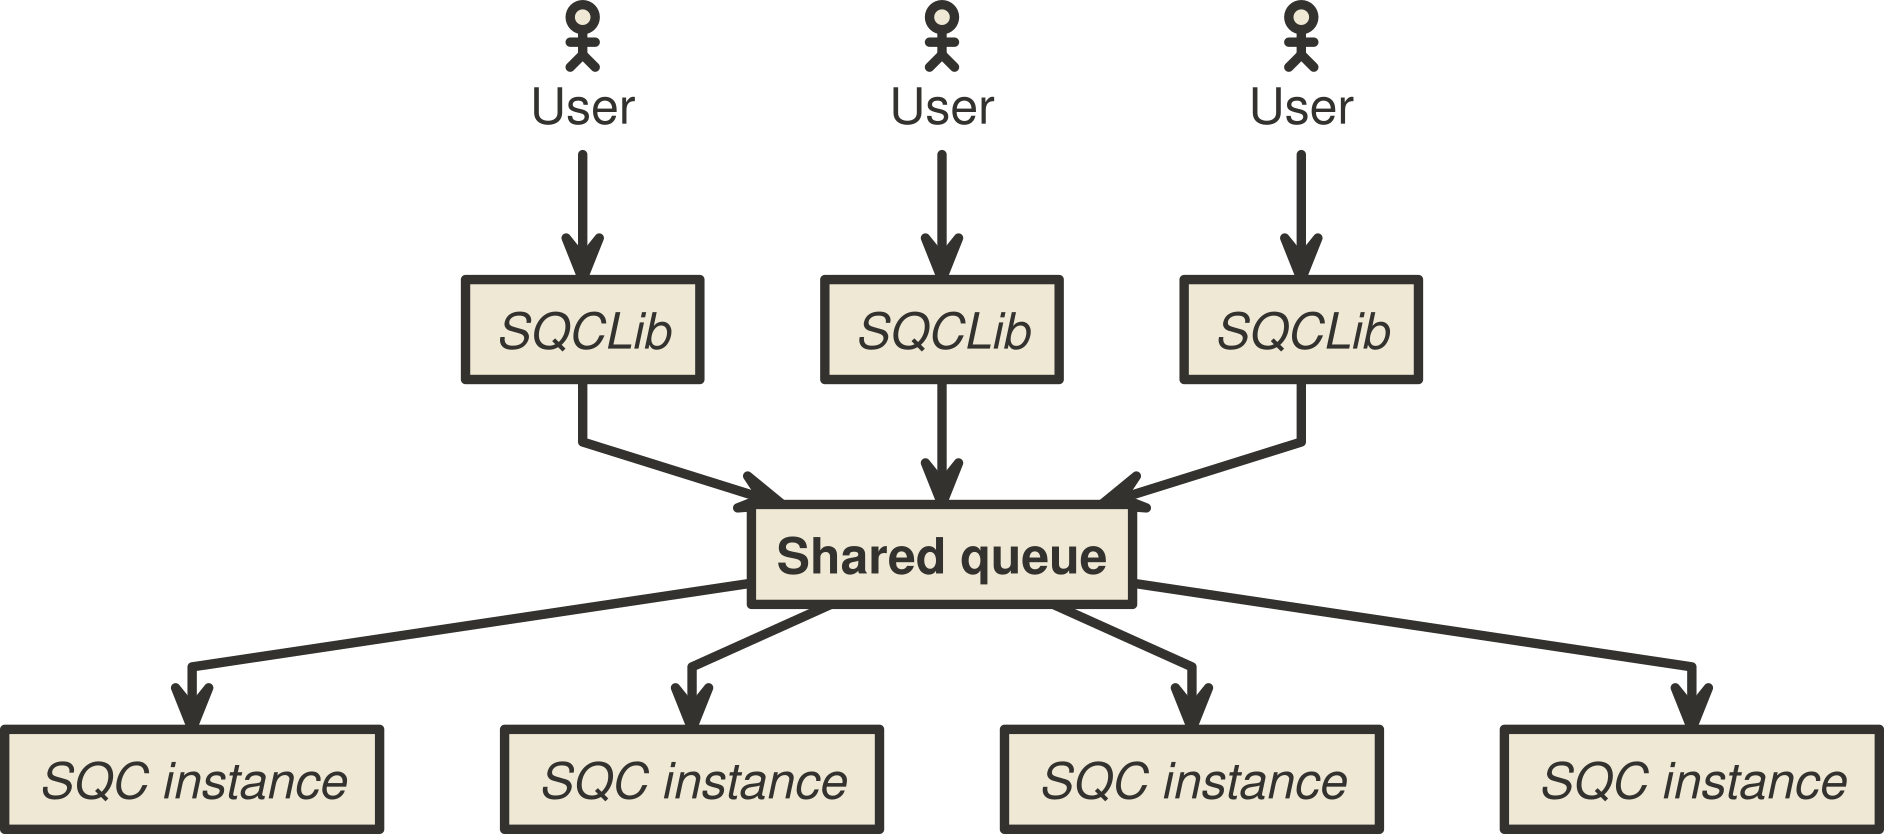
\includegraphics[width=.8\textwidth,height=.8\textheight,keepaspectratio]{img/diagram.png}
	\end{figure}
\end{frame}

\begin{frame}{Architektúra}
	\begin{figure}
		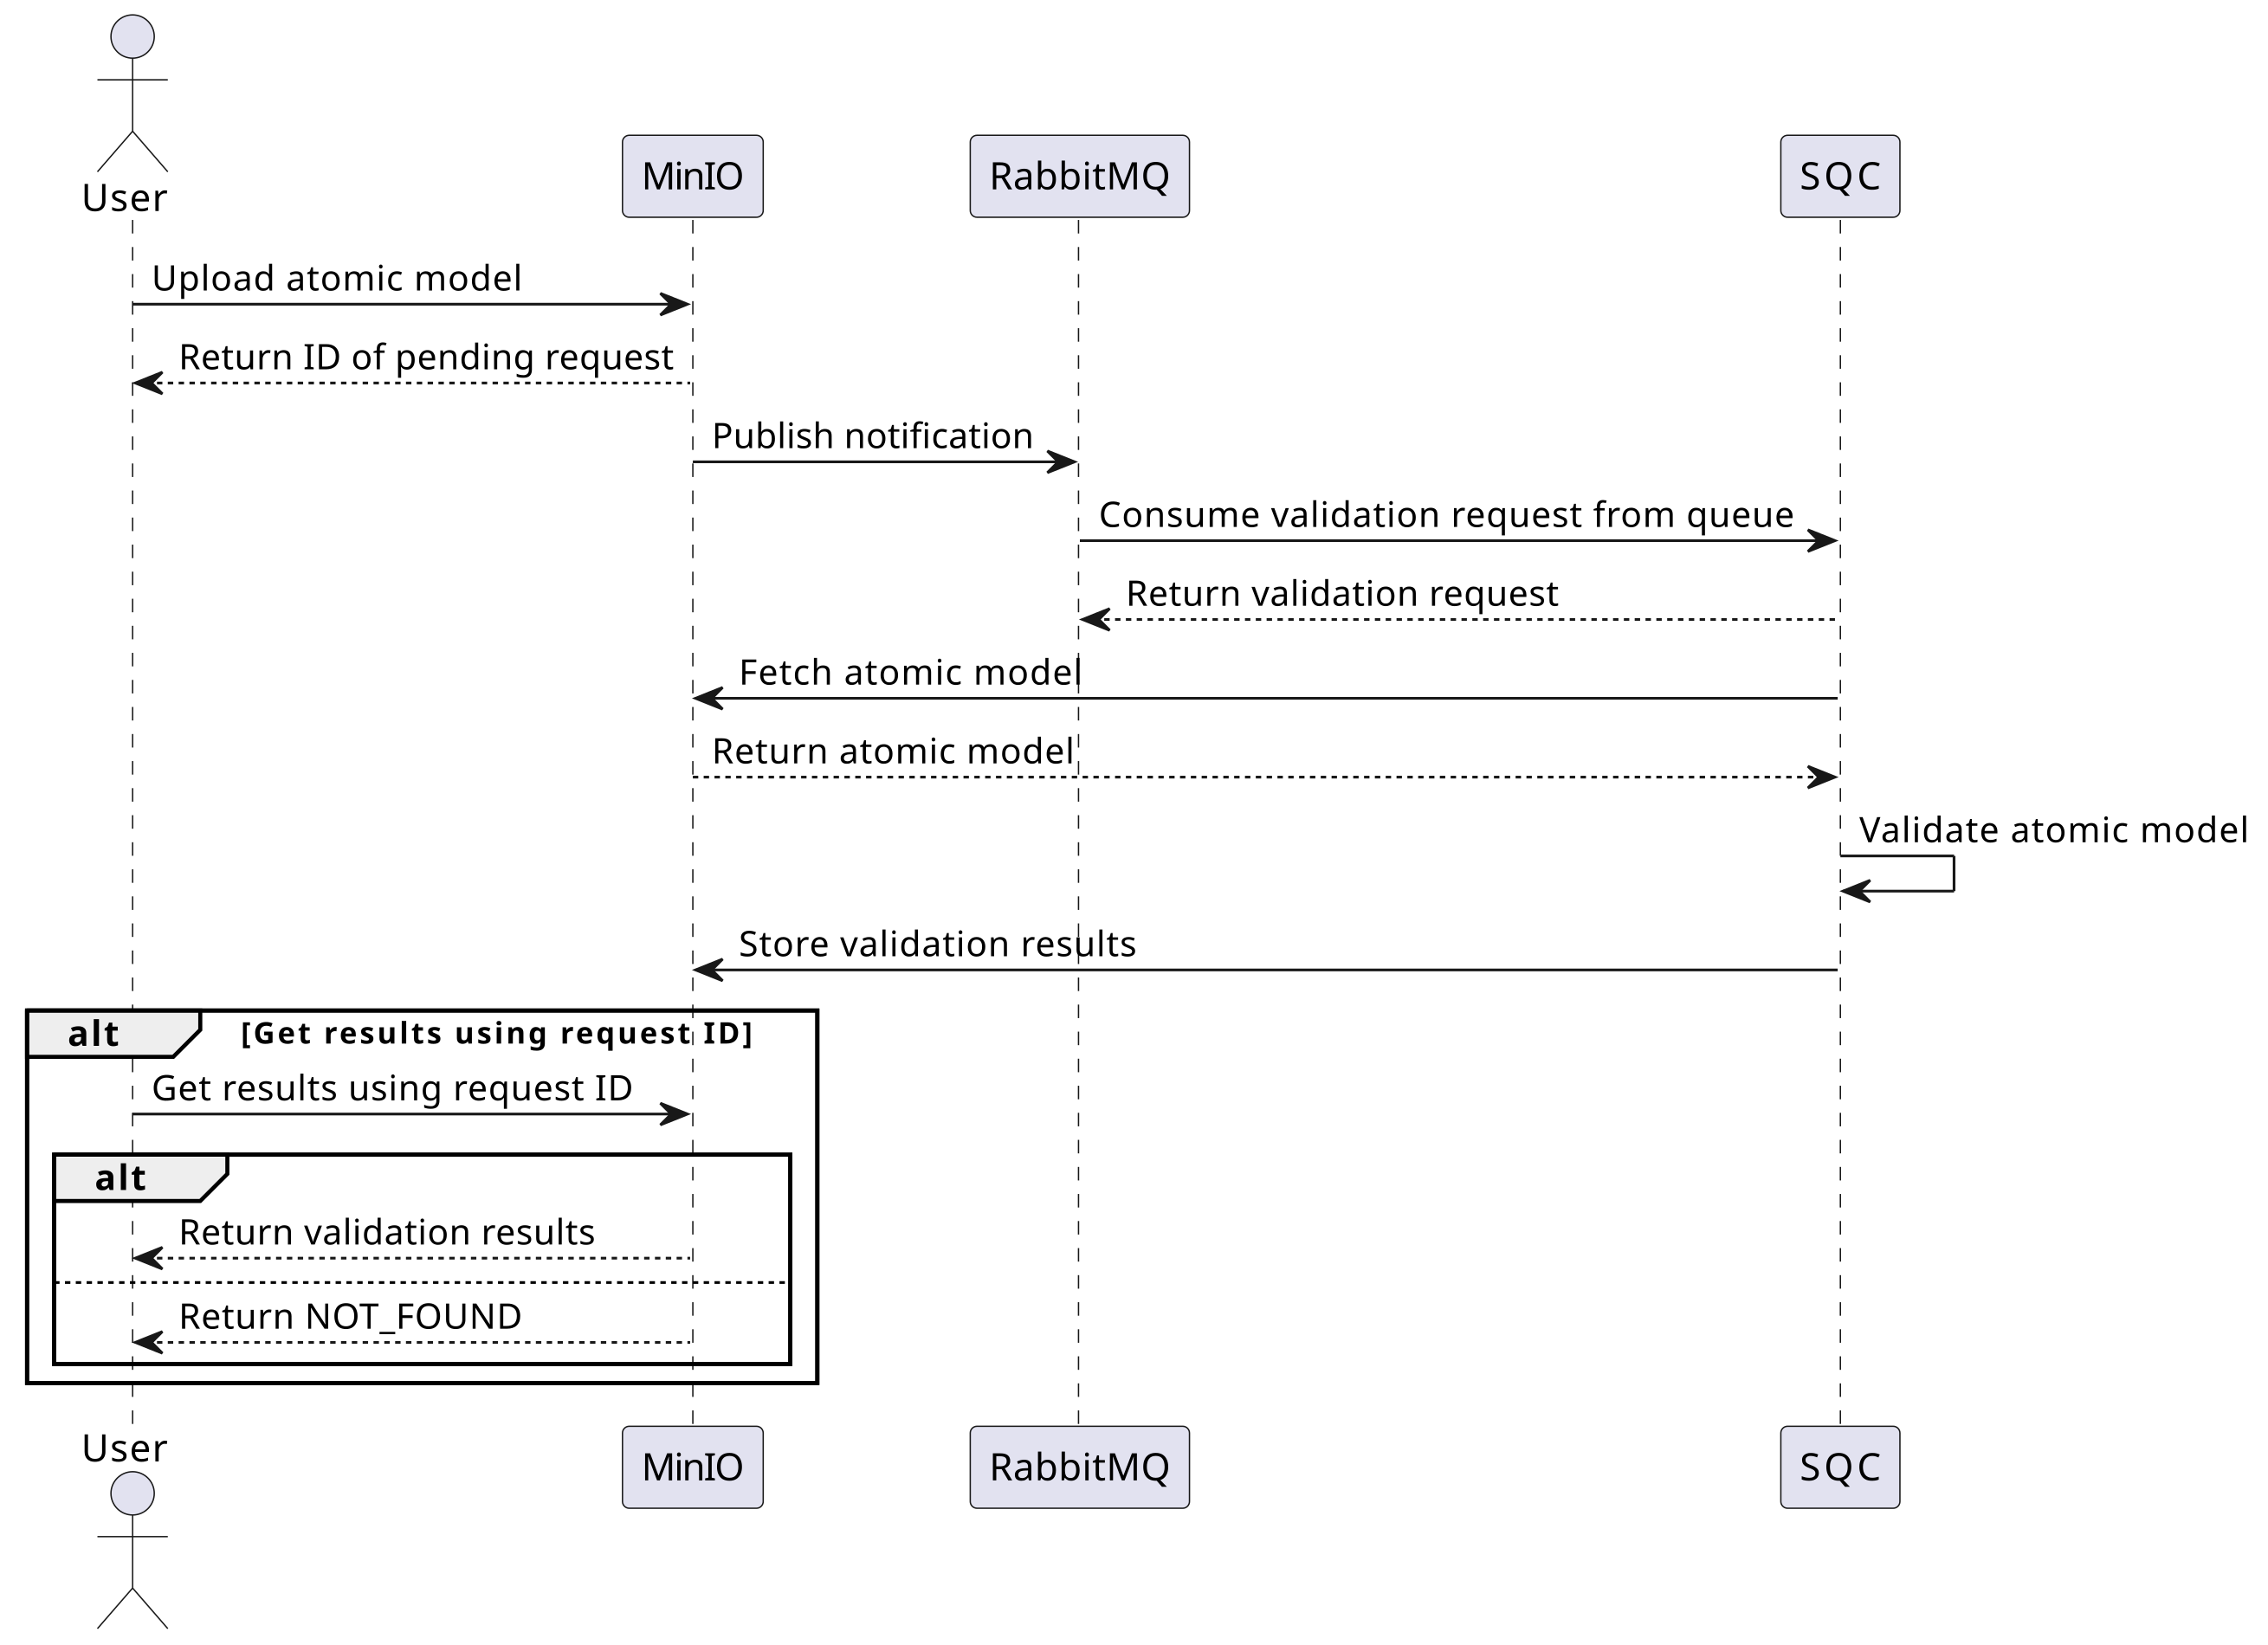
\includegraphics[width=.9\textwidth,height=.9\textheight,keepaspectratio]{img/sequence.png}
	\end{figure}
\end{frame}

\begin{frame}{Výsledky škálovania}
	\begin{figure}
		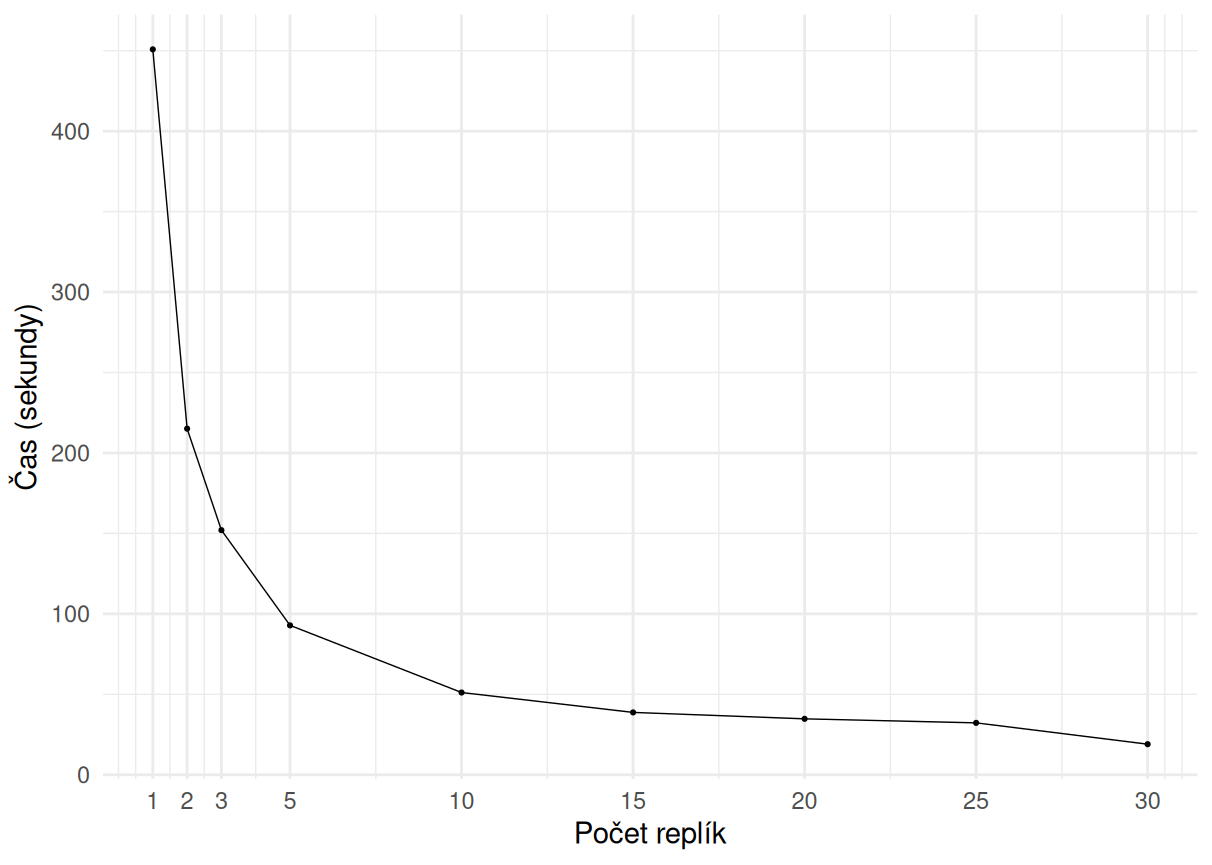
\includegraphics[width=.8\textwidth,height=.8\textheight,keepaspectratio]{img/replica-perf.png}
		\caption{Graf znázorňujúci dopad škálovania SQC inštancií na rýchlosť validácie tridsiatich štruktúr.}
	\end{figure}
\end{frame}

\begin{frame}{Nasadenie}
	\begin{itemize}
		\item Docker využitý na zjednodušenie nasadenia

		\item Všetky služby nasadené pomocou Kubernetes
		      \begin{itemize}
			      \item Cluster virtuálnej organizácie MetaCentrum
			      \item Implementácia škálovania validačného servera
			      \item Limitácia iba dostupnými prostriedkami clustera
			      \item Potenciál na škálovanie aj fronty a úložiska
		      \end{itemize}
		\item Automatizované nástrojom Ansible
	\end{itemize}
\end{frame}

\begin{frame}{Výsledky práce}
	\begin{itemize}
		\item Implementácia horizontálne škáľovateľnej validačnej služby
		      \begin{itemize}
			      \item Integruje validačné nastroje vyvinuté komunitou
			      \item Jasne definované výstupy služby
		      \end{itemize}

		\item Implementácia knižnice poskytujúcej rozhrania k službe
		      \begin{itemize}
			      \item V jazykoch Python a Bash
		      \end{itemize}

		\item Nasadenie do Kubernetes prostredí je automatizované pomocou Ansible
		\item Inštancia služby je nasadená v prostredí MetaCentra a je pripravená na použitie v projektoch SB NCBR
	\end{itemize}
\end{frame}

\makeoutro

\end{document}
